\subsection{MCMC Chain Analysis} \label{integr-synth-chain-sect}
For the analysis of the MCMC simulations, one realization of the synthetic data is chosen randomly, and the CODA package \citep{Plummer2006} is used. 

The main question to ask when monitoring an MCMC chain, is when to stop the MCMC algorithm, that is to assess when the chain has converged to the \emph{stationary} distribution. Unfortunately, there are no clear convergence markers, or theoretical guarantees to tell us when to stop the MCMC algorithm, thus, the choice is mostly empirical by using certain techniques for convergence diagnoses.

A less ambitious goal is to experimentally assess the \emph{mixing} of the chain, \ie how well the MCMC samples explore the support of the posterior distribution, and also the degree of correlation between successive random samples. Ideally, at each iteration step the samples should be \emph{independent} in order to perform Monte Carlo integration with few samples. But, MCMC samples are slightly dependent, thus the MCMC algorithm converges slowly to the target distribution; however, when the correlation between successive samples is small, the algorithm explores faster the posterior space, hence it converges faster.

\emph{Fig. \ref{trace-density-l-pic}} shows the output of the simulated chain across MCMC iterations, for the $\lambda_{k}$ parameters of the Poisson mixture model. On the left side we have the \emph{trace plots}, which show the values that the parameters took at each MCMC iteration. On the right side we have the \emph{marginal density} plot for each parameter, which is a non-parametric estimate of the distribution of the parameters in the chain. The traces have 8000 iterations, since the first 2000 iterations are discarded, \ie burn-in period.
\begin{figure}[!ht]
\begin{center}
 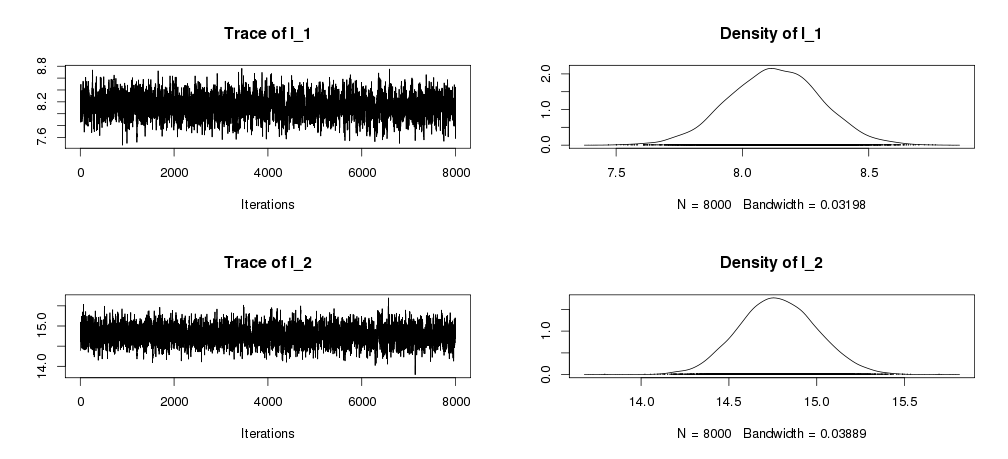
\includegraphics[scale = 0.40]{images/traceDensityL.png}
\caption{\emph{\textbf{Left:} Trace-plots for the $\lambda_{k}$ parameters of the Poisson mixture. \textbf{Right:} Corresponding marginal density plots.}}
\label{trace-density-l-pic}
\end{center}
\end{figure}

From the traces it is clear that the mixing of the chain is good, and the algorithm has found two modes of the posterior distribution where each parameter individually explores. Parameter $\lambda_{1}$ explores values around 8, whereas $\lambda_{2}$ explores values around 15, which are the true values of the generated Poisson mixtures, as explained in \emph{Section \ref{integr-synth-data-sect}}. Since, each parameter moves over a range of values around its mode and does not \emph{jump} across different modes, the marginal density plots are \emph{unimodal}.

To assess correlation between successive samples, the \emph{Auto Correlation Function (ACF)} is used. ACF measures the correlation of the values of the chain at different points in time. The \emph{lag} is the time-distance between the pair of values to be compared. The ACF for the $\lambda_{k}$ parameters of the Poisson mixture model is shown in \emph{Fig. \ref{acfL-pic}}. It is evident that the samples become uncorrelated quite fast, when $lag \approx 10$, and this allows the chain to mix well.
\begin{figure}[!ht]
\begin{center}
 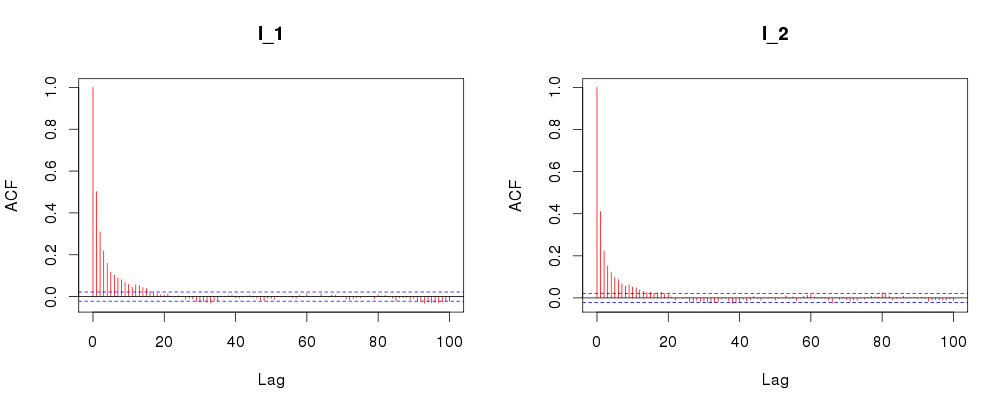
\includegraphics[scale = 0.40]{images/acfL.png}
\caption{\emph{Auto Correlation Function for the $\lambda_{k}$ parameters of the Poisson mixture. The maximum lag is set to 100.}}
\label{acfL-pic}
\end{center}
\end{figure}

The major approach for monitoring and assessing convergence of the MCMC simulation to the stationary distribution is to use multiple chains simultaneously, and then perform a statistical diagnostic test on the chains. The most widely used method is the Gelman-Rubin diagnostic \citep{Gelman1992, Brooks1997}. Basically, the method is based in analysing multiple MCMC chains by measuring whether there is a significant difference between the variance within each chain and the variance between the multiple chains. The assumption is that at convergence, the chains will have mixed well, thus the distributions of the MCMC simulations for the within and between chain variances will be very similar. Thus, we would expect that the ratio of these quantities would be around 1. The square root of this ratio is called the \emph{potential scale reduction factor (PSRF)}. 

When assessing convergence using the Gelman-Rubin diagnostic, PSRF should be close to 1 to denote chain convergence, otherwise the chain has either not reached yet the stationary distribution, or the posterior is multi-modal and different chains may converge to different local modes. A rule of thumb, if to choose really dispersed initial values between the different chains, so the MCMC chains can explore different parts of the posterior distribution as they converge to the stationary distribution.

The Gelman-Rubin diagnostic was used to assess the convergence of the $\lambda_{k}$ parameters of the Poisson mixture model, using three different MCMC chains. \emph{Fig. \ref{psrf-lambda-pic}} shows how the PSRF (or shrink factor) evolves over time. In the first few thousand iterations the shrink factor is not stable (\ie there are small bumps), but then it seems to converge, and the $PSRF \approx 1$.  
\begin{figure}[!ht]
\begin{center}
 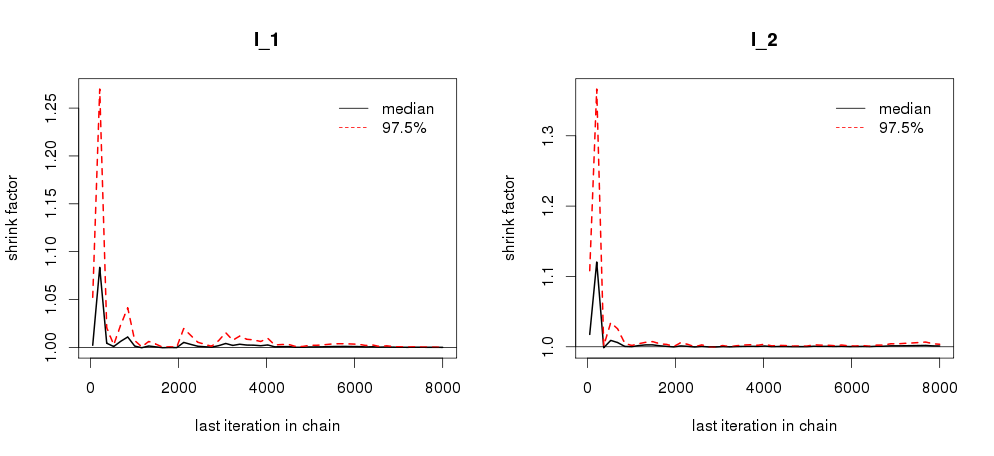
\includegraphics[scale = 0.41]{images/psrf-l.png}
\caption{\emph{Convergence of the MCMC simulations for the $\lambda_{k}$ parameters of the Poisson mixture, using the Gelman-Rubin diagnostic.}}
\label{psrf-lambda-pic}
\end{center}
\end{figure}

For brevity, only the $\lambda_{k}$ parameters of the Poisson mixture model were shown for analysis of convergence of the MCMC simulations, but similar results were obtained also for all the other parameters inferred from the BCC model. Also, the different convergence diagnostics methods were introduced without in-depth discussion. A comprehensive discussion on the convergence diagnostics for MCMC chains, including many examples, are provided in \citep{Brooks1999, Robert2009}.